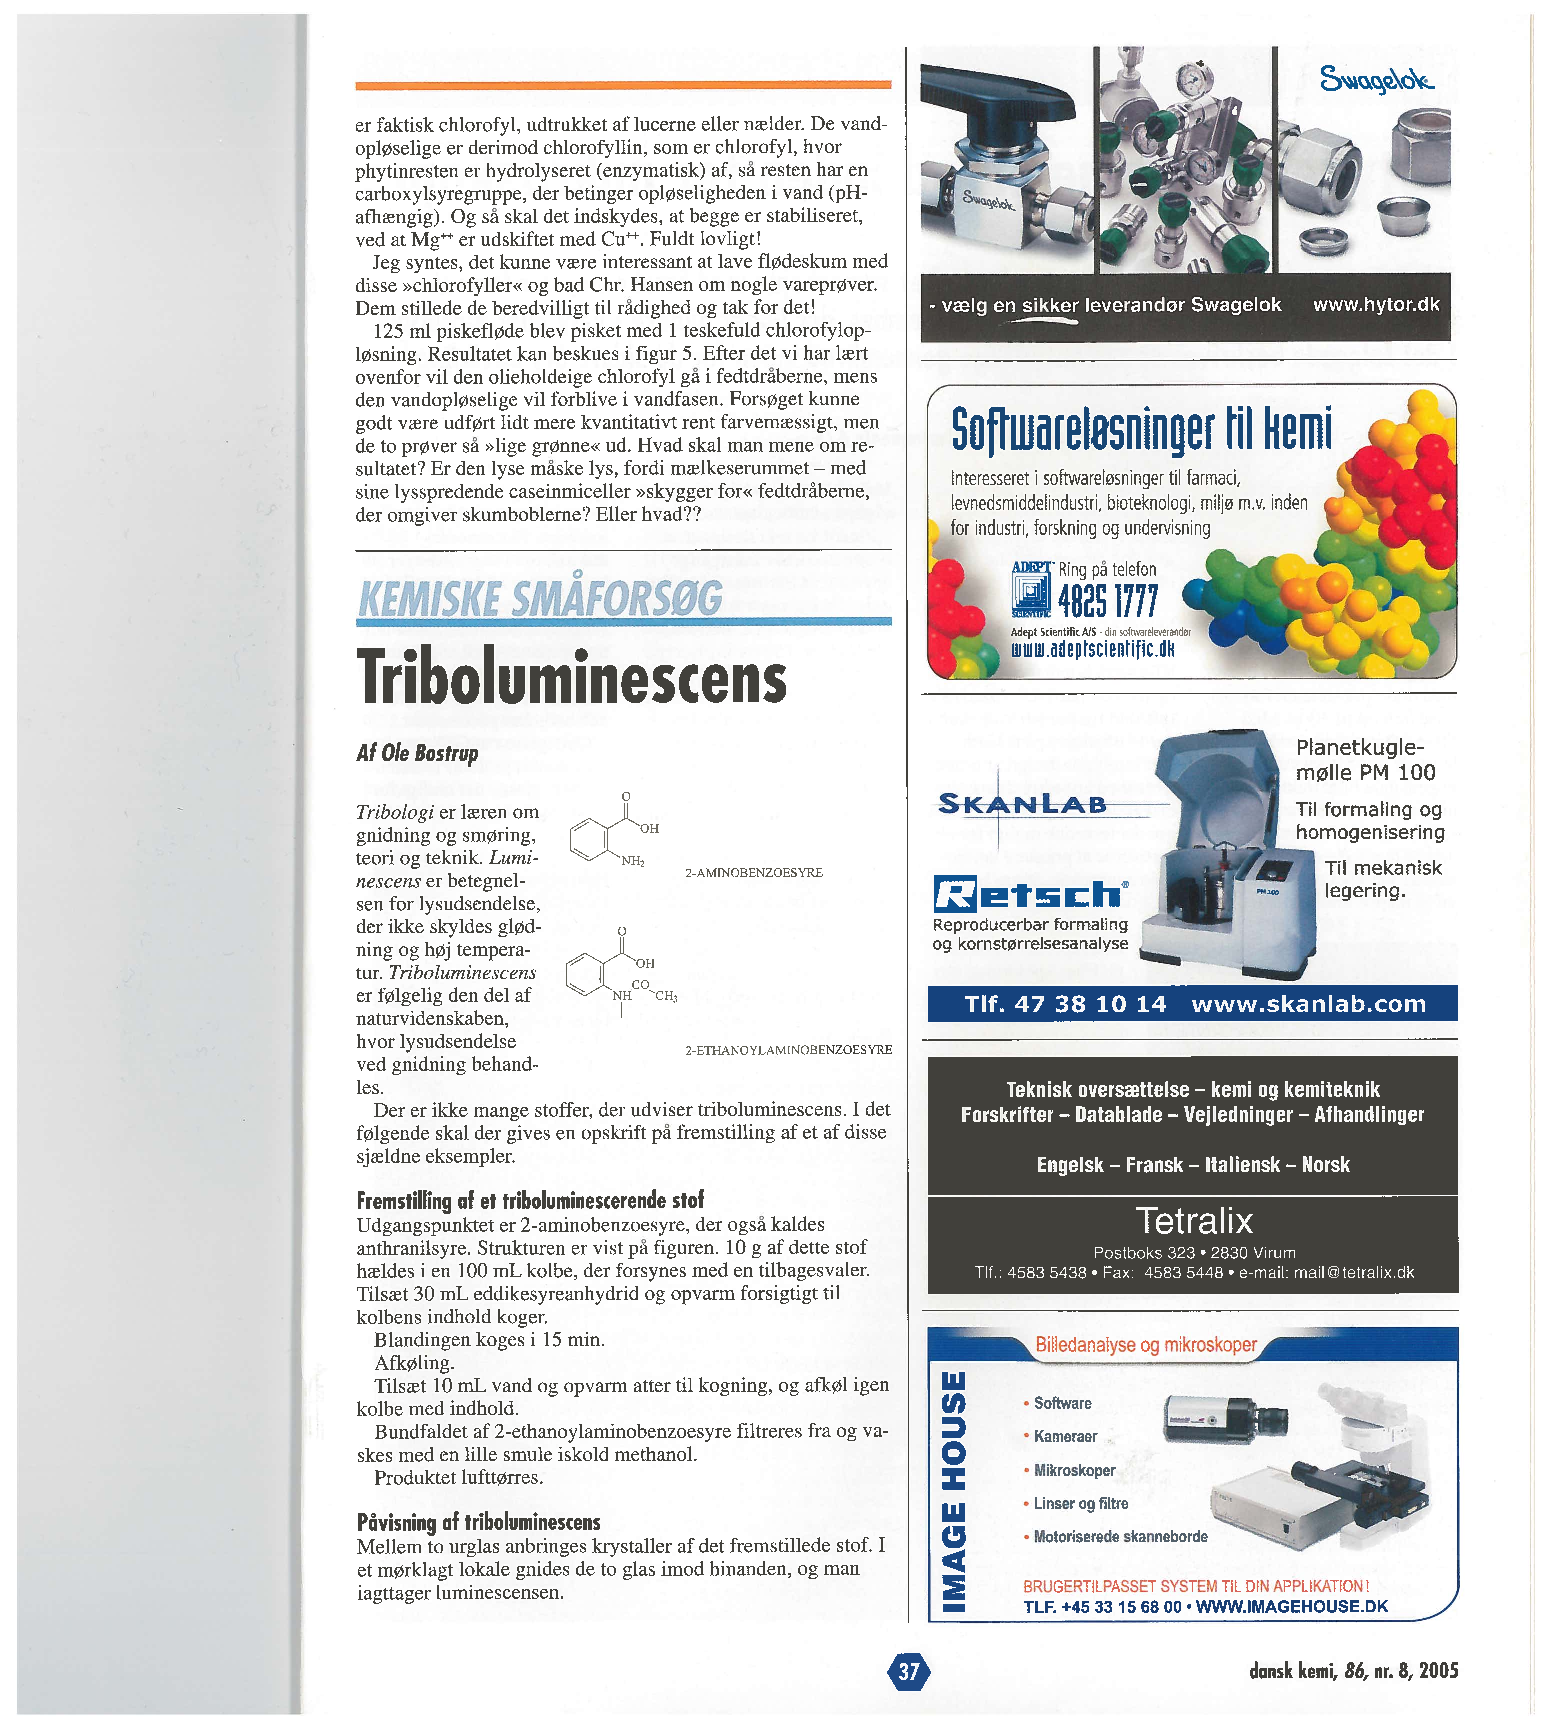
\includepdf[pages=-]{pdfs/2005-86-8-37.pdf}

\emne{Triboluminescens}

\danskkemi{Dansk kemi 86, nr. 8 2005, p 37}

Tribologi er læren om gnidning og smøring, teori og teknik. Luminescens er betegnelsen for lysudsendelse, der ikke skyldes glødning og høj temperatur. Triboluminescens er følgelig den del af naturvidenskaben, hvor lysudsendelse ved gnidning behandles.
Der er ikke mange stoffer, der udviser Triboluminescens. I det følgende skal der gives en opskrift på fremstillingen af et af disse sjældne eksempler.

\deloverskrift{Fremstilling af et Triboluminescerende stof.}
Udgangspunktet er 2-aminobenzoesyre, der også kaldes anthranilsyre. Strukturen er vist på figuren. 10 g af dette stof hældes i en 100 mL kolbe, der forsynes med en tilbagesvaler.
Tilsæt 30 mL eddikesyreanydrid og opvarm forsigtigt til kolbens indhold kooger.
Blandingen afkøles i 15 min.
Afkøling
Tilsæt 10 mL vand og opvarm atter til kogning, og afkøl igen kolbe med indhold.
Bundfaldet af 2-ethanoylamninobenzoesyre filtreres fra og vaskes med en lille smule iskold methanol.
Bundfaldet lufttørres.

\deloverskrift{Påvisning af Triboluminescens}

Mellem to urglas anbringes krystaller af det fremstillede stof. I et mørklagt lokale gnides de to glas imod hinanden, og man iagttager Luminescensen.

\chemfig{
            O% 8
     =[:270]% 7
               (
     -[:330,,,1]OH% 9
               )
     -[:210]% 3
    =_[:270]% 2
               (
     -[:330,,,1]NH_2% 10
               )
     -[:210]% 1
    =_[:150]% 6
      -[:90]% 5
     =_[:30]% 4
               (
         -[:330]% -> 3
               )
}

\chemfig{
            O% 8
     =[:270]% 7
               (
     -[:330,,,1]OH% 9
               )
     -[:210]% 3
    =_[:270]% 2
               (
     -[:330,,,1]NH% 10
      -[:270,,1]% 11
                   (
             =[:205]O% 13
                   )
         -[:320]% 12
               )
     -[:210]% 1
    =_[:150]% 6
      -[:90]% 5
     =_[:30]% 4
               (
         -[:330]% -> 3
               )
}
